% !TeX spellcheck = en_US
\documentclass[a4paper,fleqn,11pt]{article}

% header
%% Packages

% Styling TOC
\usepackage{tocloft}
\setlength\cftaftertoctitleskip{1cm}
\usepackage[nottoc]{tocbibind}

% Mathe Packages
\usepackage{amsmath,amssymb,epsfig,amsthm,amsfonts,bbm,textcomp}

% Grafiken
\usepackage[font=normalsize,aboveskip=0pt,belowskip=0pt,labelfont=bf]{caption}
\captionsetup{justification=justified,singlelinecheck=false}
\usepackage[edges]{forest}
\usepackage{tikz}
\usetikzlibrary{arrows,intersections,decorations.pathreplacing}
\usepackage[utf8]{inputenc}
\usepackage[T1]{fontenc}
\usepackage{lmodern}
\usepackage[english]{babel}

% Seiten Layout
\usepackage{float}
\usepackage[top=3cm,bottom=3cm,left=3cm,right=3cm,a4paper]{geometry}
\usepackage[onehalfspacing]{setspace}
\usepackage{color}
\usepackage{enumitem}
\usepackage{authblk}

% Fussnoten
\usepackage[flushmargin,hang]{footmisc}
\usepackage{listings}
\usepackage[hyphens]{url}
\usepackage[hidelinks]{hyperref}


% Tabellen
\usepackage{longtable} 			% Lange, mehrseitige Tabelle
\usepackage{tabularx}
\usepackage{array,hhline}
\usepackage{booktabs}			% Linien zwischen Zeilen
\usepackage{multirow}			% Verknüpfte Zellen über Zeilen hinweg
\usepackage{dcolumn}			% Erlaubt variable Orientierung am Decimalpunkt innerhalb einer Zelle
\usepackage{siunitx}

% Wir brauchen auch
\usepackage{todonotes}

% References
\usepackage{natbib}

% Paragraph spacing
\setlength{\parskip}{2ex}

% Spacing around headings
\usepackage[compact]{titlesec}





\begin{document}

% title page

% header

\pagenumbering{Roman}

\title{\huge Forecasting Swiss Exports using Bayesian \\Forecast Reconciliation}

\author[$\dagger$]{Florian Eckert}
\author[$\ddagger$]{Rob J. Hyndman}
\author[$\ddagger$]{Anastasios Panagiotelis}
\affil[$\dagger$]{\small KOF Swiss Economic Institute, ETH Zurich}
\affil[$\ddagger$]{\small Department of Econometrics and Business Statistics, Monash University}
\date{July 2019}

\maketitle
\begin{abstract}
\noindent This paper conducts an extensive forecasting study on 13,118 time series measuring Swiss goods exports, grouped hierarchically by export destination and product category.  We apply existing state of the art methods in forecast reconciliation and introduce a novel Bayesian reconciliation framework. This approach allows for explicit estimation of reconciliation biases, leading to several innovations: Prior judgment can be used to assign weights to specific forecasts and the occurrence of negative reconciled forecasts can be ruled out. Overall we find strong evidence that in addition to producing coherent forecasts, reconciliation also leads to improvements in forecast accuracy.

\noindent \textbf{JEL Classification:} C32, C53, E17\\
\noindent \textbf{Keywords}: Hierarchical Forecasting, Bayesian Forecast Reconciliation, Swiss Exports, Optimal Forecast Combination.
\end{abstract}
\clearpage




% table of contents
%\tableofcontents

%\clearpage

%\listoffigures
%\listoftables

%\clearpage

\pagenumbering{arabic}

			




% 2. Model	
\section{Introduction}
\label{sec:intro}
Forecasts of exports can support the decisions of a number of economic agents including policy-makers, \todo{other examples}.  These forecasts may be of interest in their own right but also as inputs into forecasting other important macroeconomic quantities such as exchange rates and GDP growth\todo{maybe find references}.  In many cases economic agents are not interested in the forecast of total exports but of some disaggregate series.  For instance, a trader trying to forecast the exchange rate between the Swiss Franc and Chinese Yuan will be more interested in Swiss exports to China rather than total Swiss exports to all countries.  A Swiss manufacturer of watches trying to manage its inventories will be more interested in the exports of Swiss watches rather than the total exports of all goods.  This paper is motivated by a real world problem \todo{maybe something in here about who has asked you to do this}, namely forecasting 13,118 individual time series. Each of these time series measures exports of Swiss goods, some series measure the exports of particular product categories to particular export destinations, while other series are aggregates of these series.

The data we consider are an example of {\em hierarchical time series}; as a result of their aggregation structure, both the actual data and all future realisations of the data will adhere to some linear constraints \todo{general reference to fpp}.  Our Swiss export data are disaggregated geographically by export destination into regions such as Europe, North America or Australia. These regional aggregates are then disaggregated further by country. Swiss exports are also disaggregated into product categories such as precision instruments, textiles or vehicles and then further into subcategories such as road, rail, air and water vehicles. As such, our data have the structure of a so-called grouped hierarchy \citep{Hyndman2016}. Figure \ref{fig:tree} gives a simple example of grouped structure with $k = 3$ levels, $m = 9$ series in total and $q = 4$ series at the most disaggregate or `bottom' level.
\begin{figure}[H]
	\centering
	\begin{forest}
		before packing={
			forked edges,
		}
		[{$Y_0$}
		[{$Y_{A}$}
		[{$Y_{A1}$}]
		[{$Y_{A2}$}]
		]
		[{$Y_{B}$}
		[{$Y_{B1}$}]
		[{$Y_{B2}$}]
		]
		]
	\end{forest}\hspace{1cm}
	\begin{forest}
		before packing={
			forked edges,
		}
		[{$Y_0$}
		[{$Y_{1}$}
		[{$Y_{A1}$}]
		[{$Y_{B1}$}]
		]
		[{$Y_{2}$}
		[{$Y_{A2}$}]
		[{$Y_{B2}$}]
		]
		]
	\end{forest}
	\vspace{0.4cm}
	\caption[Simple Example of a Grouped Hierarchy]{\textbf{Simple Example of a Grouped Hierarchy.}}
	\label{fig:tree}
\end{figure}

Since it is known that all future realisations of the data will adhere to the constraints implied by the aggregation structure, a desirable property of any forecasts is that they also respect these constraints.  Such forecasts are referred to as {\em coherent forecasts}.  In the case of Swiss exports, incoherent forecasts are problematic because they lead to contradictory conclusions, and non-aligned decision making.  

There are a number of strategies that can be employed to ensure coherent forecasts.  Earlier literature reduced the issue of producing coherent forecasts as one of selecting a specific level of the hierarchy. For instance the `bottom-up' approach \citep{Gross1990} achieves coherence by producing forecasts for the bottom level series only and then summing these up according to the hierarchical structure.  A major shortcoming of this approach is that disaggregate series tend to be very noisy and there is a high risk of model misspecification.  For example features such as seasonality may be difficult to identify in the bottom level series, despite being clearly present in the aggregate series.  To address this shortcoming a `top-down' approach was proposed \citep[see][and references therein]{Athanasopoulos2009}.  Here, the forecast of the top level series is disaggregated according to the historical or forecast proportions of lower levels. A weakness of the top-down approach is information loss because the time series characteristics at lower levels are not taken into account. A compromise is given by the `middle-out' approach, where the forecasts at an intermediate level of the hierarchy are summed up to get the higher levels and disaggregated to obtain lower level predictions.  A major shortcoming of the middle-out (and also top-down) method is that they are not easily applied to the grouped hierarchical structure present in our data.

In response to these shortcomings, over the past decade there has been a tendency towards producing forecasts for all series in the hierarchy rather than only at a single level.  These are referred to as {\em base} forecasts.  Depending on how they are produced, base forecasts may no longer adhere to aggregation constraints.  {\em Forecast reconciliation}, introduced by \cite{Hyndman2011} performs an ex-post adjustment to base forecasts to produce a new set of coherent forecasts. This adjustment effectively combines predictions from all levels and in doing so `hedges' against misspecification error across all levels.  There is now substantial theoretical and empirical evidence that forecast reconciliation can significantly improveme forecast accuracy~\citep[see][and references therein]{Wickramasuriya2015}. The first main contribution of our own paper is therefore to apply existing reconciliation methods to the problem of forecasting Swiss export data.

Despite their success, forecast reconciliation methods suffer a number of shortcomings, some of which hold in general, and others which arise due to the idiosyncracies of our dataset.  First, forecast reconciliation can induce negative forecasts even when the base forecasts are non-negative, something that is clearly problematic when forecasting quantities that must be non-negative such as exports.   Second, an important theoretical assumption to ensure the optimality of forecast reconciliation is that forecasts are unbiased prior to reconciliation.  Often this assumption will fail to hold in practice.  Third, existing reconciliation methods combine forecasts in a way that is backwards looking, combining models using weights that depend on the inverse of past variation of forecast errors.  There are several instances where this approach breaks down for our dataset.  One is the case of exports to small trading partners which are zero for most and in some cases all of the obsevations in the training sample.  These can forecast almost perfectly by a naive forecast of zero and the presence leading to small (or even no) variation in forecast errors and numerically unstable forecast reconciliation.  Another case where the backward looking nature of reconciliation breaks down is when forecasters have information that a forecasting models may break down even if it has performed well in the past. An example of this in our dataset is a structural break induced by the reclassification of electricity as a good rather than a service.  Finally, the backwards-looking nature of existing reconciliation methods also makes it difficult to exploit information from the entire predictive density of a forecast target.\\

In light of this, the second major contribution of our paper is to extend existing forecast reconciliation in a way that addresses the shortcomings described in the previous paragraph. The main innovation is to convert the general reconciliation equation into a panel regression. Rather than using a single vector of point forecasts, we draw samples from the predictive densities of the base forecast models. This panel regression is estimated using Bayesian Markov Chain Monte Carlo algorithms. Our approach has a number of benefits relative to the existing methodology. First, reconciliation biases in the base forecasts are made explicit by introducing fixed effects into the panel regression structure. This overcomes a major weakness of existing approaches which require base forecasts to be unbiased to ensure that reconciliation is optimal. Second, we propose a mechanism for down-weighting the influence of particular series irrespective of past forecasting performance. This is valuable if forecasters have strong judgmental reasons for believing that a particular model will work particularly well in the future and other base forecasts will be less reliable. Third, under our approach, the weights used in reconciliation can depend on the variances of the predictive density rather than in-sample forecast errors. Existing approaches essentially determine weights based on estimates of the unconditional variance. Our innovation is therefore particularly promising for forecasting models that allow for conditional heteroskedasticity. Fourth, the Bayesian estimation procedure conveniently allows the incorporation of prior information to solve issues such as the occurrence of negative reconciled forecasts. 

The remainder of the paper is structured as follows. Section~\ref{sec:data} introduces in detail the Swiss export data, using modern techniques for exploring and visualising high-dimensional time series.  Section~\ref{sec:methods} introduces in detail both existing forecast reconciliation as well as our novel Bayesian approach.  Section \ref{sec:appl} conducts an extensive forecast evaluation that compares our proposed method with existing reconciliation techniques. Section~\ref{sec:conc} concludes.

\clearpage


\section{Data}\label{sec:data}
We use a comprehensive dataset containing exports of Swiss goods. All time series cover a period from 1988 to 2018 in monthly frequency and are denominated in Swiss francs. They are not adjusted for seasonalities or calendar effects. The data can be grouped by export destination and product category. The geographical hierarchy consists of 8 regions, aggregated from 245 countries and dependent territories. The categorical hierarchy follows a national nomenclature covering 12 main economic groups and 48 subgroups\footnote{Precious metals, precious and semi-precious stones, works of art and antiques are generally omitted in business cycle research due to volatility and structural breaks.}. This leads to a grouped hierarchy with $m = 13,118$ series containing nonzero entries in total and $q = 9,483$ series at the bottom level. Figure \ref{fig:area} shows the historical development of the regional and categorical hierarchies.
\begin{figure}[H]
	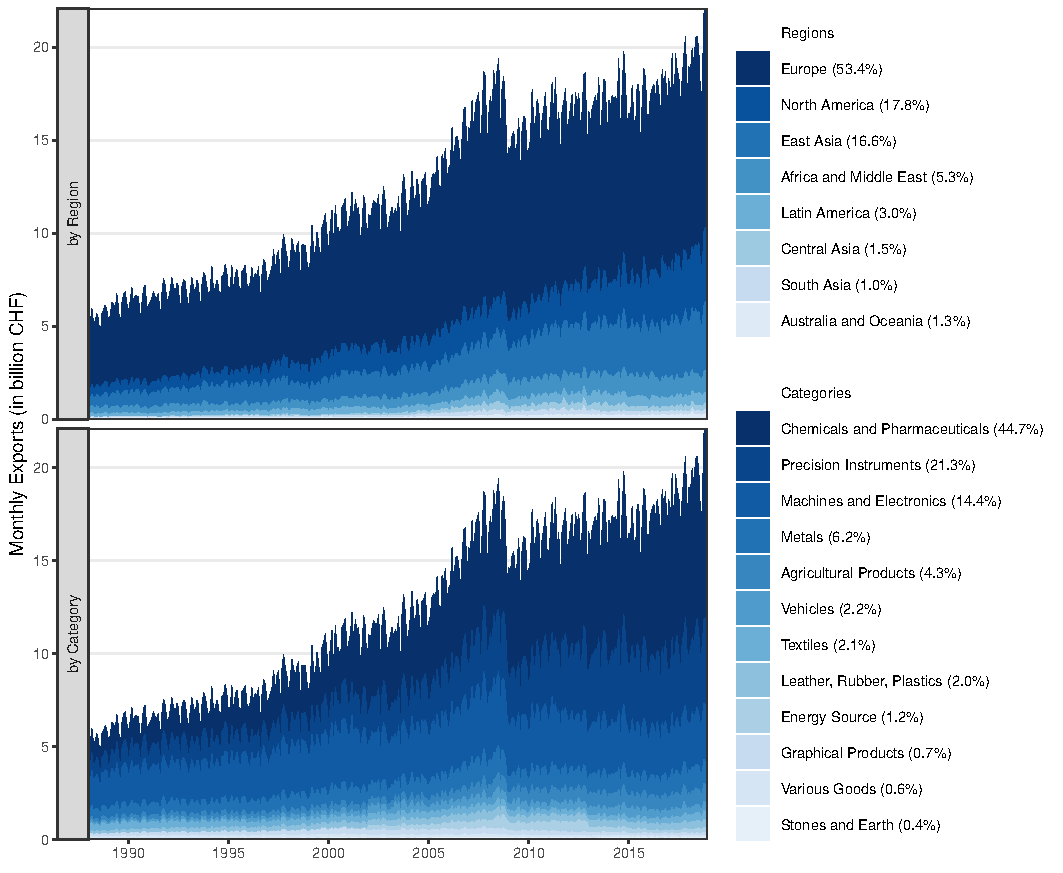
\includegraphics[width=\textwidth]{fig/fig_area}
	\caption[Contribution to Swiss Exports of Goods]{\small{\textbf{Contribution to Swiss Exports of Goods}. \textit{Nominal values, not adjusted for seasonalities or calendar effects. Average export shares of the year 2018 in parentheses.}}}\label{fig:area}
\end{figure}
As a result of its status as a small open economy in a rapidly globalizing world, nSwiss exports have increased significantly since the late 1980s. Accounting for more than half of total exports, Europe is a key market for Swiss goods. Increasingly larger shares of exports also go to North America and East Asia with around 17\% each in 2018. Exports to Africa and the Middle East, Latin America, Central and South Asia and Australia account only for about 10\% combined.

The hierarchical grouping by categories is more evenly distributed, but has been subject to greater shifts in its composition. The most important categories are `Chemicals and Pharmaceuticals', `Precision Instruments' and `Machines and Electronics'. Figure \ref{fig:treemap} shows the changes in composition between 1988 and 2018.
\begin{figure}[H]
	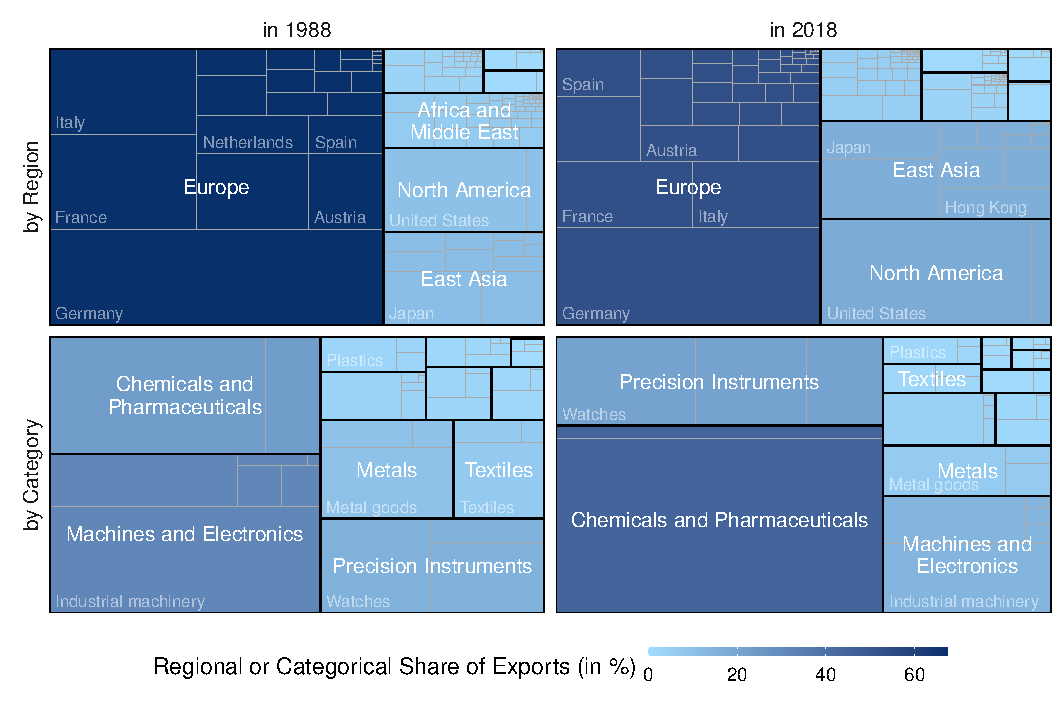
\includegraphics[width=\textwidth]{fig/fig_treemap}
	\caption[Regional and Categorical Composition of Swiss Goods Exports]{\small{\textbf{Regional and Categorical Composition of Swiss Goods Exports.}}}\label{fig:treemap}
\end{figure}
The two hierarchical groupings are quite different. The geographic hierarchy with 8 groups and 245 subgroups is very wide. With a majority of the export volume going to European countries, it is nevertheless highly concentrated. This has changed slightly in the past 30 years as the relative share of exports to the rest of the world has increased. The categorical hierarchy on the other hand is rather narrow with 12 groups and 48 subgroups. Compared to the regional hierarchy, the export volume is however more evenly distributed, even though an increasing concentration, particularly in chemicals and pharmaceuticals, can be noted.\\

Due to the aggregation involved, top level series are usually less noisy and exhibit more predictable characteristics such as seasonality or trend. Following \cite{Kang2017}, it is possible to construct a measure of predictability for each time series by estimating principal components from a number of time series features that are commonly associated with better predictability. This includes measures such as the strength of seasonality, trend, spectral entropy and serial correlation.  On the vertical axis, Figure \ref{fig:feature} shows the first principal component, which accounts for a large share of the variation in these predictability features.
\begin{figure}[H]
	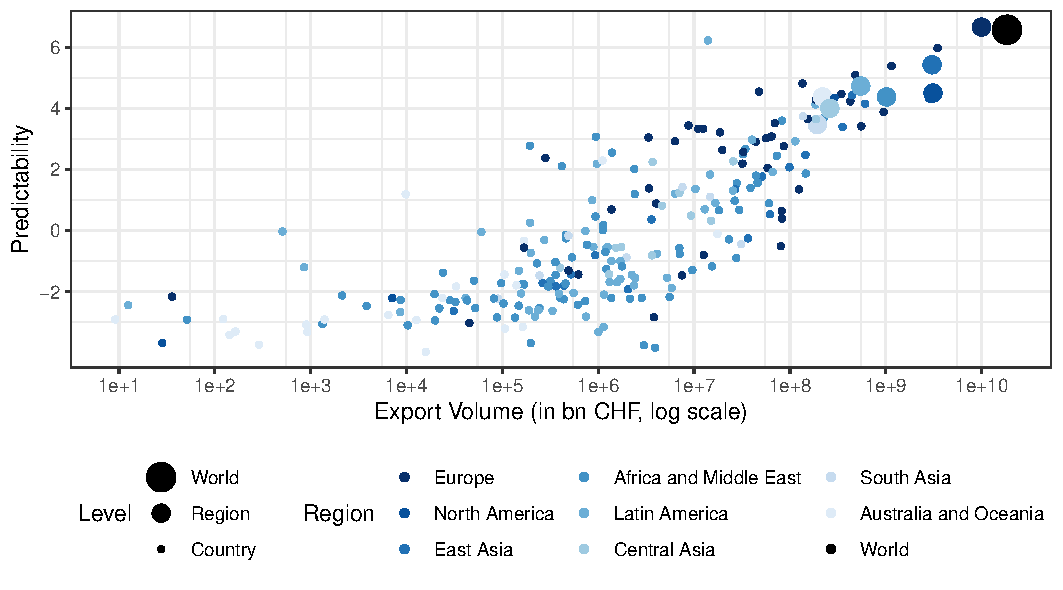
\includegraphics[width=\textwidth]{fig/fig_confetti}
	\caption[Predictability of Different Levels in a Hierarchy]{\textbf{Predictability of Different Levels in a Hierarchy.}\textit{ Predictability is defined as the first principal component of a large number of time series characteristics.}} \label{fig:feature}
\end{figure}
It is evident that there exists a strong correlation between predictability and export volume. This implies that larger series and consequently those at the top of a hierarchy are easier to forecast. This finding strengthens the claim that reconciliation biases for top level series should be smaller in relative terms than those at the bottom level.\\

\section{Forecast Reconciliation}
\label{sec:methods}

\subsection{Existing Forecast Reconciliation Methods}
	
In order to encode the aggregation constraints in a hierarchy, we define $Y_t$ to be an $m$-vector that stacks observations at time $t$ from all series, $Y_{k,t}$ to be a subvector of $Y_t$ containing only the $q$ bottom level series at time $t$ and $S$ to be an $m\times q$  aggregation matrix.  In the simple grouped hierarchy shown in Figure~\ref{fig:tree}, these are given by
\begin{align*}
	\underset{(m\times 1)}{Y_t} = \begin{bmatrix}
		\ Y_0\ \ \\
		\ Y_A\ \ \\
		\ Y_B\ \ \\
		\ Y_1\ \ \\
		\ Y_2\ \ \\
		\ Y_{A1}\ \ \\
		\ Y_{A2}\ \ \\
		\ Y_{B1}\ \ \\
		\ Y_{B2}\ \ 
	\end{bmatrix} \quad \underset{(m\times q)}{S} &=
	\begin{bmatrix}
		\ 1 & 1 & 1 & 1 \ \ \\
		\ 1 & 1 & 0 & 0 \ \ \\
		\ 0 & 0  & 1 & 1\ \ \\
		\ 1 & 0 & 1 & 0 \ \ \\
		\ 0 & 1 & 0 & 1\ \ \\
		\ 1 & 0 & 0 & 0 \ \ \\
		\ 0 & 1 & 0 & 0 \ \ \\
		\ 0 & 0 & 1 & 0 \ \ \\
		\ 0 & 0 & 0 & 1\ \ 
	\end{bmatrix} \quad \underset{(q\times 1)}{Y_{k,t}} = \begin{bmatrix}
		\ Y_{A1}\ \ \\
		\ Y_{A2}\ \ \\
		\ Y_{B1}\ \ \\
		\ Y_{B2}\ \ 
	\end{bmatrix} 
\end{align*}
Here, and in general, the matrix $S$ is defined so that $Y_t = S Y_{k,t}$ holds for all realized data. 
	
\cite{Hyndman2011} considered a framework whereby forecasts for all $m$ series and at all levels are produced, referring to these as `base forecasts'.  To reconcile these base forecasts, the following regression structure was assumed.
\begin{align}
	Y_t(h) &= S\beta_{h} + e_t(h)
	\label{eq:regstruct}
\end{align}
where $Y_t(h)$ is an ($m \times 1$) vector containing the h-periods-ahead base forecasts at time $t$ for each level in the hierarchy, $\beta_{h}$ represents the true expected value of the bottom level series and the error term $e_t(h)$ has mean zero and covariance matrix $\Sigma_h$. Reconciled forecasts are given by $Sb_{h}$, where $b_h$ is an estimate of $\beta_{h}$ that combines information about forecasts at all levels. It can be estimated using the following regression equation.
\begin{align}
	\label{eq:reg}
	b_{h} &= \left(S'W_h^{-1}S \right)^{-1} S'W_h^{-1}Y_t(h)
\end{align}
This choice minimizes the generalized Euclidean distance between $Y_t(h)$ and the reconciled forecasts $Sb_{h}$ with respect to $W_h$. Reconciliation is also guaranteed to reduce the distance to the eventual realization targeted by a forecast. There are several potential choices for $W_h$. Letting $W_h=I$ corresponds to an ordinary least squares estimate.  Alternatively, a high degree of heteroskedasticity in the error terms motivates a diagonal $W_h$ or weighted least squares approach. Under so called `variance scaling', weights are the variances of in-sample $h$-step ahead forecast variances, and forecasts with less accurate historical performance are down-played in reconciliation.  Another alternative is the `nseries' approach due to \cite{Athanasopoulos2017}, whereby weights are based on the number of series aggregated at each node.  More recently, the `MinT' approach was developed by \cite{Wickramasuriya2015} to allow for a $W_h$ that is not diagonal and exploits the covariances between the $h$-step-ahead reconciled forecast errors. The nomenclature MinT refers to the fact that this approach minimizes the trace of the covariance matrix of reconciliation errors.\\



\subsection{Bayesian Framework}
\label{sec:model}

We now propose a new methodology for forecast reconciliation.  The main insight is to recognise that additional information about the uncertainty surrounding a measure of central tendency, can be provided by generating base forecasts from density forecasts.   In the spirit of \cite{Kapetanios2015} or \cite{Cesur2016}, the predictive distributions of the $m$ base forecast models are approximated by drawing samples of size $n$. Possible sources for obtaining these draws are posterior predictive distributions from Bayesian forecasting models, bootstrap aggregating, model pooling or simply by sampling from a fitted model. This results in $n$ vectors $\hat{y}_{i}$, each of length $m$, that contain a draw $i$ from each predictive distribution.\footnote{Since every forecast horizon is reconciled independently, the time subscripts are dropped from now on to simplify notation.} 

This allows the regression model from Equation~\ref{eq:regstruct} to be recast as a panel regression.  The error term consists of two components, a prediction error $e_{i}$ and a reconciliation bias $\alpha$. The latter can be interpreted as a fixed effect that is unique to each forecasted variable. In other terms, $\alpha$ is the difference between the unreconciled forecast mean $\hat{y}$ and the reconciled forecast mean $\tilde{y}$. The interpretation of $\beta$ depends on the definition of $S$, but in general it estimates the mean of the bottom level reconciled forecasts. The following equation can then be used to model the forecast reconciliation.
\begin{align}
\label{eq:main}
\begin{tabular}{ccccccccc}
	$\hat{y}_i$ & $=$ & $\alpha$ & + &$S$ & $\times$ & $\beta$ & $+$ & $e_i$ \\
	$\scriptscriptstyle (m\times 1)$ & & $\scriptscriptstyle (m\times 1)$  & & $ \scriptscriptstyle (m\times q) $ & & $\scriptscriptstyle (q\times 1)$ & & $\scriptscriptstyle (m\times 1)$
\end{tabular}
\end{align}
where $e$ follows a normal distribution with mean zero and covariance matrix $\Sigma$. The reconciliation problem in (\ref{eq:main}) can be expressed as a system of seemingly unrelated regressions (SUR) to account for cross-equation correlations. Since the explanatory variables are the same for each equation, it is a special case of the SUR model in \cite{Zellner1962}. However, the parameters are impossible to estimate directly because of perfect multicollinearity in the regressors $I_m$ and $S$. This is quite intuitive since there is more than one unique way to reconcile incoherent forecasts. Following \cite{Farebrother1978}, the regression is partitioned in order to separate the parameters that cause multicollinearity and they are estimated in separate Gibbs sampling steps. The distribution of the reconciled forecasts can be obtained by sampling from the posterior predictive distribution conditional on $\alpha$ being equal to zero.
\begin{align*}
p(\tilde{y}\ |\ \alpha = 0,\hat{y}, S) &= \iint p(\tilde{y}\  |\  \alpha = 0,\beta,\Sigma,\hat{y},S)\ p(\alpha = 0,\beta,\Sigma\  |\  \hat{y},S)\ d\beta\ d\Sigma
\end{align*}
The joint posterior distribution of $\alpha$, $\beta$ and $\Sigma$ is obtained by combining a prior belief on the parameters with the likelihood according to Bayes' theorem.
\begin{align}
p(\alpha, \beta, \Sigma\ |\ \hat{y}, S) \propto p(\hat{y}, S\ |\ \alpha, \beta, \Sigma) \times p(\alpha, \beta, \Sigma)
\end{align}
The likelihood function of the data is given by
\begin{align*}
p(\hat{y},S\ &|\ \alpha,\beta,\Sigma) \propto \frac{1}{|\Sigma|} \exp\left[-\frac{1}{2} \sum_i  (\hat{y}_i - \alpha - S\beta)'\Sigma^{-1}(\hat{y}_i - \alpha - S\beta)\right]
\end{align*}
The joint posterior distribution is accordingly given by
\begin{align*}
p(\alpha,\beta,\Sigma\ |\ \hat{y},S) & \propto \frac{1}{|\Sigma|} \exp\left[-\frac{1}{2} \sum_i  (\hat{y}_i - \alpha - S\beta)'\Sigma^{-1}(\hat{y}_i - \alpha - S\beta)\right] \\
&\times \exp \left[-\frac{1}{2}(\alpha - a_0)'A_0^{-1}(\alpha - a_0)\right] \\
&\times \exp \left[-\frac{1}{2}(\beta - b_0)'B_0^{-1}(\beta - b_0)\right] \\
&\times \frac{1}{|\Sigma|(v_0 - m - 1)} \exp \left[-\frac{1}{2} tr(R_0^{-1}\Sigma^{-1}) \right]
\end{align*}
The Bayesian approach has the advantage that uncertainty surrounding the parameters $\alpha$, $\beta$ and $\Sigma$ is taken into account. Following \cite{Percy1992}, we get the marginal distributions by approximating the joint posterior distribution via Gibbs sampling from the conditional distributions.  Convergence is usually achieved very quickly, irrespective of the starting values. It can be verified by testing for stability in the recursive means of the Markov chains. A sufficiently large sample of draws from the posterior predictive distribution of $\tilde{y}$ is saved and evaluated to get summary statistics such as mean and variance of the reconciled forecasts.\\

\noindent\textbf{Step 1: Draw $\beta$ conditional on $\alpha,\Sigma,\hat{y},S$}\\
The parameter $\beta$ is the mean of the bottom level forecasts, given an appropriate aggregation matrix $S$. The conditional posterior distribution is then given by
\begin{align}
\beta\ |\ \alpha,\Sigma,\hat{y} &\sim N(b_1,B_1)
\end{align}
where $B_1 = \left(\sum_i S'\Sigma^{-1}S + B_0^{-1}\right)^{-1}$ and $b_1 = B_1 \left(\sum_i S'\Sigma^{-1} (\hat{y}_i - \alpha) + B_0^{-1}b_0\right)$. Unless there is reason to believe otherwise, the priors $b_0$ and $B_0$ should be chosen as uninformative as possible. In some cases, this regression approach leads to negative values in the reconciled bottom level forecasts. This might be a concern since many applications such as sales or exports do not allow for negative observations. Using a truncated normal prior, this issue can be resolved in an uncomplicated fashion by simply discarding draws of $\beta$ that contain negative entries during the sampling process.\\

\noindent\textbf{Step 2: Draw $\Sigma$ conditional on $\alpha,\beta,\hat{y},S$}\\
$\Sigma$ is the covariance matrix of the prediction errors. While $\Sigma$ is not singular by definition because the forecasts in $\hat{y}_{i}$ are not reconciled, it might be near-singular if the base forecasting models are estimated jointly or if the draws are reordered following \cite{Jeon2018}. In the latter case $\Sigma$ can be drawn from an inverse Wishart distribution.
\begin{align}
\Sigma\ |\ \alpha,\beta,\hat{y} \sim W^{-1}(v_1,R_1)
\end{align}
where $v_1 = v_0 + n$ and $R_1 =  \left( R_0^{-1} + \sum_i (\hat{y}_i - \alpha - S \beta)'(\hat{y}_i - \alpha - S \beta) \right)^{-1}$. It is useful to set an almost uninformative prior with $v_0$ and $R_0$ very close to zero, which introduces a tiny bit of noise into the reconciled forecasts. This has negligible impact on the posterior distribution, but ensures that $\Sigma$ is nonsingular in the case where a base forecast has no variation. A possible simplification is to draw the variances equation-by-equation from an inverse gamma distribution.\\

\noindent\textbf{Step 3: Draw $\alpha$ conditional on $\beta,\Sigma,\hat{y},S$}\\
Because the reconciliation regression is an ill-posed problem, it is necessary to impose additional restrictions on the reconciliation biases $\alpha$ in order to achieve identification. The conditional distribution of $\alpha$ can be expressed equivalently by concentrating out $\beta$ in the following reconciliation identity.
\begin{align}
	\label{eq:prior1}
	\alpha &= \frac{1}{n}\sum_i \hat{y}_i - S\beta
\end{align}
In order to eliminate $\beta$ from equation (\ref{eq:prior1}), both sides are multiplied by a projection matrix $P$. The reconciliation biases depend greatly on the definition of this projection matrix and alternative choices for $P$ will be discussed in section \ref{sec:weighting}. Using $P = S(S'S)^{-1}S'$ implies an orthogonal projection onto the coherent subspace. The resulting terms are then subtracted from both sides of equation (\ref{eq:prior1}).
\begin{align}
	\label{eq:prior2}
	(I_m - P)\ \alpha &= (I_m - P)\ \frac{1}{n}\sum_i \hat{y}_i  
\end{align}
It is useful to define the idempotent residual maker $M = I_m - P$. Since $M$ is not invertable due to the presence of multicollinearity, equation (\ref{eq:prior2}) cannot be solved for $\alpha$. Our identifying assumption is that $\alpha$ lies in the span of $M$ in which case $M\alpha = \alpha$. For $P=S(S'S)^{-1}S'$, this implies that the direction of the reconciliation bias is orthogonal to the coherent subspace.  This solves the identification problem and leaves the reconciliation biases as a function of the data and the residual maker $M$. This result is again very intuitive since the reconciliation biases are the residuals from a regression of the base forecasts on the aggregation matrix.
\begin{align}
\alpha &= M\left(\frac{1}{n}\sum_i \hat{y}_i\right)
\end{align}
 Having identified the system in that way, the prior variance $A_0$ is allowed to be uninformative and the prior mean $a_0$ is a zero vector. A numerically stable conditional posterior for $\alpha$ is therefore given by
\begin{align}
	\label{eq:alpha}
	\alpha\ |\ \beta,\Sigma,\hat{y} &\sim N(a_1,A_1)
\end{align}
where $A_1 = M\left(\frac{\Sigma}{n}\right)M'$ and $a_1 = M\left(\frac{1}{n}\sum_i \hat{y}_i\right)$. 


\subsection{Bias Weighting}
\label{sec:weighting}
The definition of the projection matrix $P$ is crucial for the estimated parameters. Figure \ref{fig:weights} demonstrates the impact of different projections on the estimated reconciliation biases. It features identical unreconciled forecasts of a simple hierarchy with $m=3$ series, where $Y_A + Y_B = Y_0$. For each series a sample is drawn from the predictive forecasts density, assumed to be $N(4,2)$ for $Y_A$ (shown in blue), $N(6,1)$ for $Y_B$ (shown in purple), and $N(16,3)$ for $Y_0$ (shown in yellow). The horizontal axis shows draws from the unreconciled base forecasts, which are clearly incoherent. The vertical axis on the other hand shows the means of the reconciled forecasts. The diagonal line shows values where the means of base and reconciled forecasts are equal.
\begin{figure}[H]
	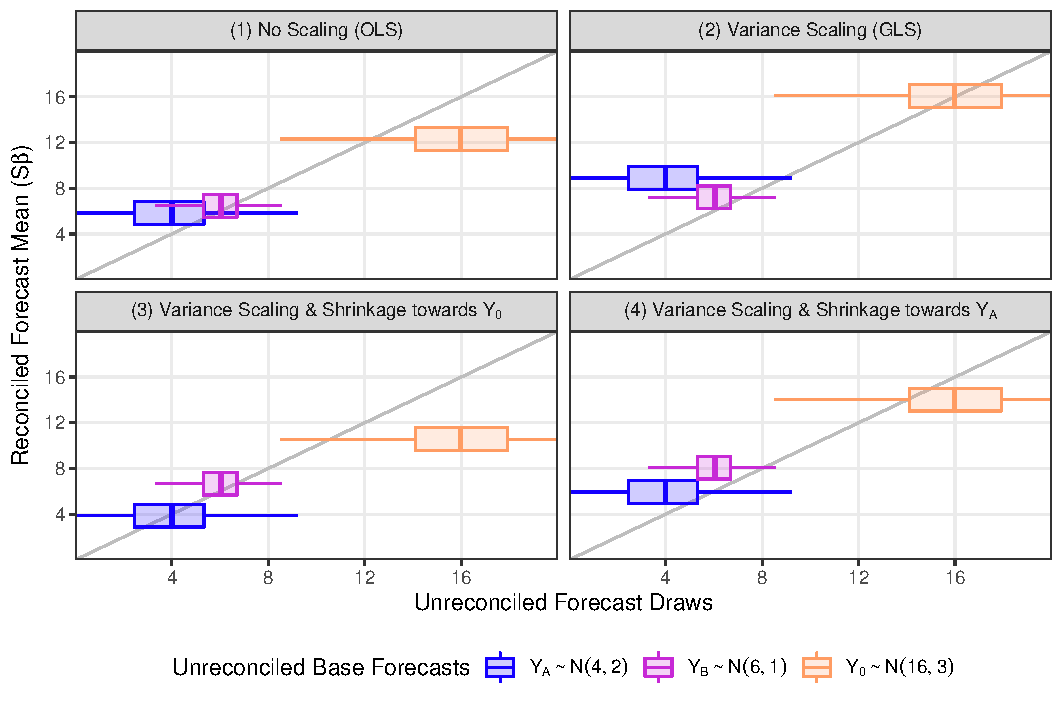
\includegraphics[width=\textwidth]{fig/fig_biases}
	\caption[Weighting Schemes]{\textbf{Weighting Schemes.} \small{\textit{The grey line indicates where the unreconciled base forecasts on the x-axis are equal to reconciled forecast means on the y-axis.}}}\label{fig:weights}
\end{figure}
Each panel corresponds to a different choice of $P$. Using $P = S(S'S)^{-1}S'$ corresponds to the orthogonal projection in an ordinary least squares regression. Subfigure (1) shows that the forecast biases for each margin are treated equally, consequently the means of $Y_A$ and $Y_B$ are adjusted upwards while the mean of $Y_0$ is adjusted downwards. Using $P = S(S'\Sigma^{-1}S)^{-1}S'\Sigma^{-1}$ implies that the reconciliation biases are weighted with the inverse of their corresponding forecast variances. This leads to a smaller adjustment in $Y_B$ (the reconciled and base means are close) relative the others since it is more accurate.\\

Even though it is intuitive to weight the reconciliation biases using the predictive accuracy of the corresponding base forecasts, this can be generalized to different weighting schemes. There may exist prior information on the reliability of certain models or the requirement to fix some forecasts at specific values. This could be due to better data availability, higher suitability of a particular model or subjective judgment of the forecaster. Weighting can be achieved by using a projection matrix $P= S(S'(\Lambda\Sigma\Lambda')^{-1}S)^{-1}S'(\Lambda\Sigma\Lambda')^{-1}$ that includes a diagonal matrix of weights $\Lambda$. It might be of interest to selectively shrink some reconciliation biases in $\alpha$ towards zero by decreasing the corresponding entry in $\Lambda$. At the same time, it is necessary to increase the remaining elements such that they are able to capture the higher reconciliation biases at their level of the hierarchy. This is achieved by keeping constant the total dispersion of the  multivariate normal distribution $\Lambda\Sigma\Lambda'$. A common measure is the generalized variance described in \cite{Mustonen1997} and defined as the determinant of a covariance matrix. The weighting matrix $\Lambda$ is therefore always constructed such that the product of the diagonal elements remains constant at 1. This in turn ensures that the total dispersion of $\Lambda\Sigma\Lambda'$ remains equal to the total dispersion of the unweighted $\Sigma$ for all $\Lambda$. Subfigures (3) and (4) shrink the reconciled forecasts of $Y_0$ and $Y_A$ towards their base forecasts.\\

It is important to note that the likelihood is invariant to these choices. Besides the shrinkage of specific reconciliation biases towards zero, there are several other weighting methods conceivable.  Possible approaches include the weighting of each series by its level in the hierarchy or by to the number of series at each node in the hierarchy. This allows for the emulation of the `nseries', `bottom-up', `middle-out' and `top-down' results. A convenient feature of this is that the `middle-out' and `top-down' shrinkage work also for grouped time series, which is not the case in the standard approach. \\

\clearpage


\section{Reconciliation of Export Forecasts}
\label{sec:appl}

\subsection{Setup}
The large hierarchy of Swiss goods exports is used to test the Bayesian reconciliation framework and various competing methods. Each month from 1995 to 2015, forecasts for all series in the hierarchy are calculated for the next 36 months. For each of the 13,118 series, forecasts are calculated from three models: An autoregressive integrated moving average model (ARIMA), an exponential smoothing state space model (ETS) and a seasonal random walk model (RW). As described in \cite{Hyndman2008}, the model for each series is parametrized automatically based on the Akaike information criterion. In order to get samples from the predictive densities, $n = 1000$ sample paths are simulated from each fitted model using Gaussian errors. With the exception of the volatile period during the Great Recession, the ARIMA and ETS approaches outperform the Random Walk on average for series at every level and forecasting horizon. All results in the following subsection will therefore rely on ARIMA forecasts.\footnote{A comparison of forecasting methods, horizons and accuracy measures can be found in appendix \ref{sec:robust}.}\\

These incoherent forecasts are then reconciled using several basic single level and optimal combination methods. The single level techniques include bottom-up, top-down and middle-out methods. The latter two can only be used for non-grouped time series and are therefore tested on the regional and categorical hierarchies separately. The optimal combination methods used are the ordinary and weighted least squares, nseries, MinT and Bayesian reconciliation (BSR). Draws from the predictive distributions are obtained by sampling from the fitted models assuming normality of the errors. If aggregation of the prediction errors is necessary, they are weighted with their respective export share.\\

The resulting coherent forecasts are evaluated using several accuracy measures such as the root mean squared error (RMSE), mean absolute percentage error (MAPE) and mean absolute scaled error (MASE). The method of \cite{Diebold1995} is used to test whether reconciled forecasts are significantly more accurate than unreconciled forecasts. The Diebold-Mariano test checks for significance in the difference between two squared forecast errors at various forecasting horizons, accounting for serial correlation in the squared error loss. In addition, another significance test is used to compare the mean squared errors directly. Since the prediction errors are assumed to be normally distributed, the ratio between mean squared errors of an unreconciled forecast and a specific reconciled forecast has an $F$-distribution with degrees of freedom corresponding to the number of errors. This allows us to test for equality of the unreconciled and reconciled mean squared prediction errors.\\


\subsection{Comparative Results}
This section provides empirical evidence for the benefits of optimal hierarchical combination. It compares the performance of different reconciliation methods and explores which data characteristics profit in particular from hierarchical combination.\\
 
\noindent\textbf{Benefits of Hierarchical Combination.} Figure \ref{fig:rmse} shows the accuracy of forecasts, defined as the mean squared error of the base forecasts relative to the mean squared errors of the coherent forecasts from each method. Higher bars indicate therefore better forecast performance. The 95\% confidence interval shows the acceptance region of an $F$-test for equality of the mean squared errors. It is worth noting that reconciliation methods and bottom-up forecasts are the only techniques that allow for coherence across all levels of a grouped hierarchy. Top-down and middle-out reconciliations are not applicable in the case of grouped time series.

It is evident that single level methods do not consistently improve forecasting accuracy. The bottom-up and middle out methods fare reasonably well for the top level series, but fail to outperform the unreconciled forecasts at lower levels and are sometimes even significantly worse. Optimal combination on the other hand tends to outperform the base forecasts especially for top and intermediate level series. Especially the methods using variance scaling, such as MinT, WLS and BSR, work very well at all levels.
\begin{figure}[H]
	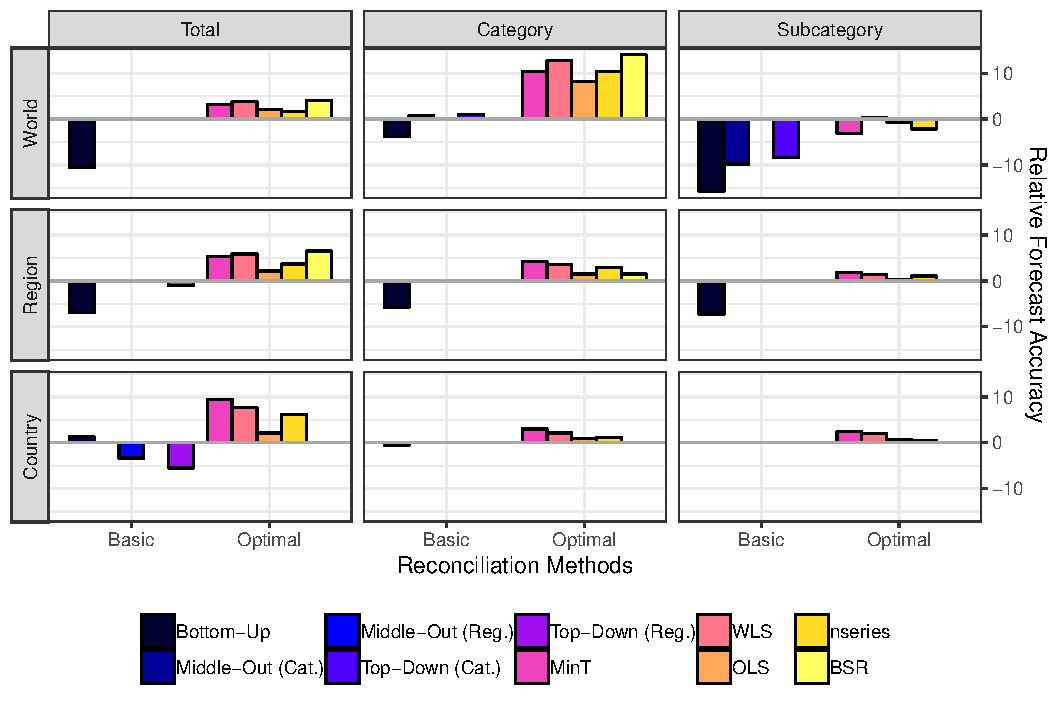
\includegraphics[width=\textwidth]{fig/fig_eval_rmse_relative}
	\caption[Relative Accuracy of Reconciliation Methods]{\textbf{Relative Accuracy of Reconciliation Methods.} \small{\textit{Higher bars indicate better forecasts relative to the unreconciled case. The zero line shows the accuracy of unreconciled predictions, with a 95\% confidence interval for the ratio of mean squared errors to be one. Average of all forecast horizons.}}} \label{fig:rmse}
\end{figure}


\noindent\textbf{Comparison of Combination Methods.} It is also instructive to look at the development of the relative forecasting accuracy over time in figure \ref{fig:rmse_time}. Even though the variance scaling methods are more accurate on average, they do not consistently outperform the unreconciled forecasts. It also appears that MinT, WLS and BSR perform fairly similar over time. For the top level series, the benefits of reconciliation accrued mostly during times of global economic distress and corresponding appreciations of the Swiss franc.

The biggest gains can be observed during the early 2000s recession following the burst of the dot-com bubble, the global financial crisis and the following sovereign debt crisis in Europe, and the sudden appreciation of the Swiss franc after the Swiss National Bank stopped supporting the currency peg to the Euro in early 2015. Interesting is the forecasting accuracy after January 2002, when electrical energy was reclassified as a good instead of a service. The structural break in the time series leads to misspecified models, but the rigid structure imposed by the hierarchy increases forecast accuracy substantially relative to the unreconciled case.\\
\begin{figure}[H]
	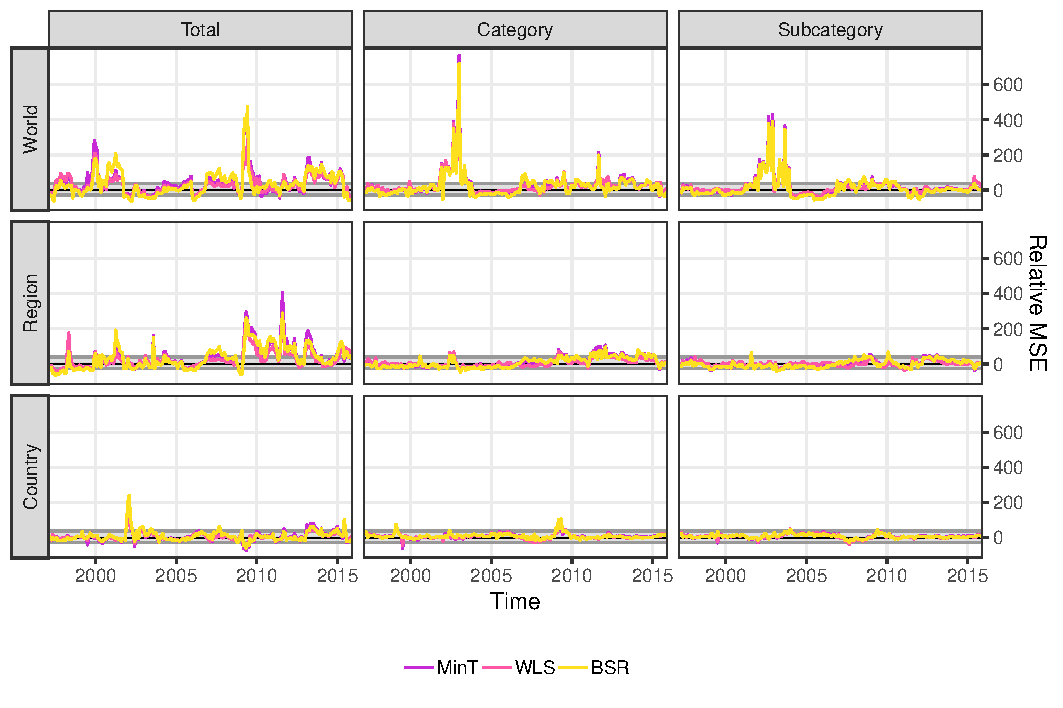
\includegraphics[width=\textwidth]{fig/fig_eval_rmse_time}
	\caption[Relative Accuracy of Reconciliation Methods over Time]{\textbf{Relative Accuracy of Reconciliation Methods over Time.} \small{\textit{Higher lines indicate better forecasts. Zero line shows the accuracy of unreconciled predictions, with a 90\% confidence interval for the ratio of mean squared errors to be one. Base forecasts are generated using ARIMA models. Average of all forecast horizons.}}} \label{fig:rmse_time}
\end{figure}

\noindent\textbf{Significance of Results.} In order to check whether the accuracy improvements are significant, one-sided Diebold-Mariano tests are used for the top-level series. Figure \ref{fig:dmtest} shows the p-values when testing for equality of reconciled and unreconciled forecasts. The alternative hypothesis is that the accuracy of reconciliation methods is greater. With the exception of the middle-out approach, single level methods are not significantly more accurate than the unreconciled forecasts at all horizons. Optimal combinations are more significant than single level methods and .. \todo{Why is OLS so much better here?}

\begin{figure}[H]
	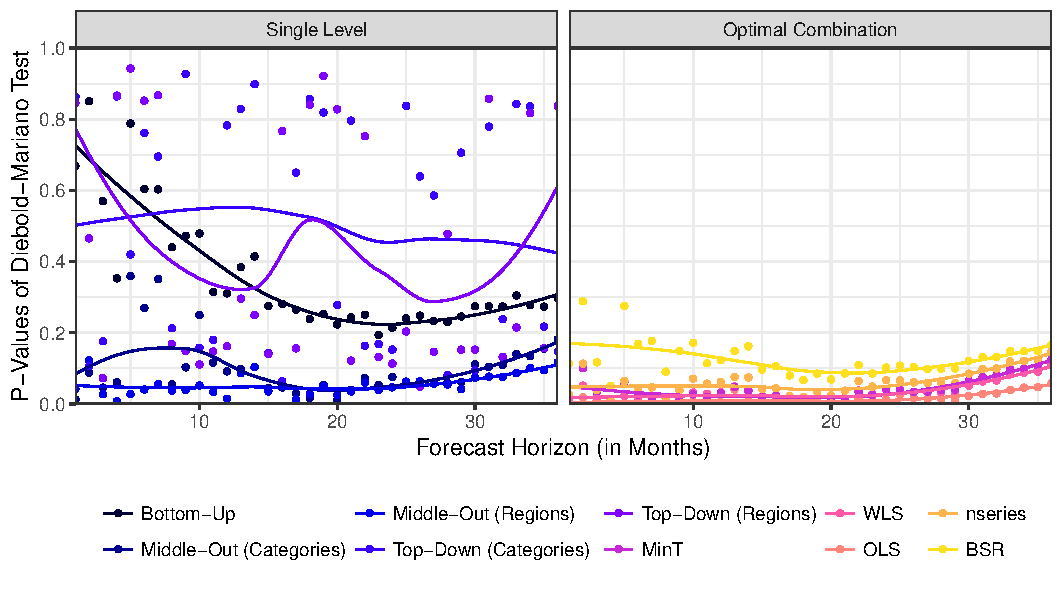
\includegraphics[width=\textwidth]{fig/fig_dm}
	\caption[Significance of Forecast Accuracy Improvements]{\textbf{Significance of Forecast Accuracy Improvements.} \small{\textit{Test for top-level total exports series, where points indicate p-values of Diebold-Mariano test for greater accuracy of reconciled versus unreconciled forecasts. Lines indicate locally estimated scatterplot smoothed (LOESS) p-values.}}} \label{fig:dmtest}
\end{figure}


\noindent\textbf{Implications for Data Characteristics.} Another way to dissect the results is to identify which time series see the greatest gains in forecast accuracy from using reconciliation. Figure \ref{fig:eval_regions} provides an overview of the relative forecast accuracy by geographical classification, using the Bayesian reconciliation framework. It is again obvious that reconciled forecasts are on average more accurate than in the unreconciled case, but not in every instance. It appears that series with a larger export volume benefit most from reconciliation. Forecasts of exports to countries in Europe, North America and East Asia are almost entirely better off than in the unreconciled case, whereas forecasts of exports to countries with a lower share, such as the islands in Oceania, tend to be worse off. In addition, time series at higher levels in a hierarchy do not necessarily profit more from reconciliation than their corresponding subcategories.
 \begin{figure}[H]
	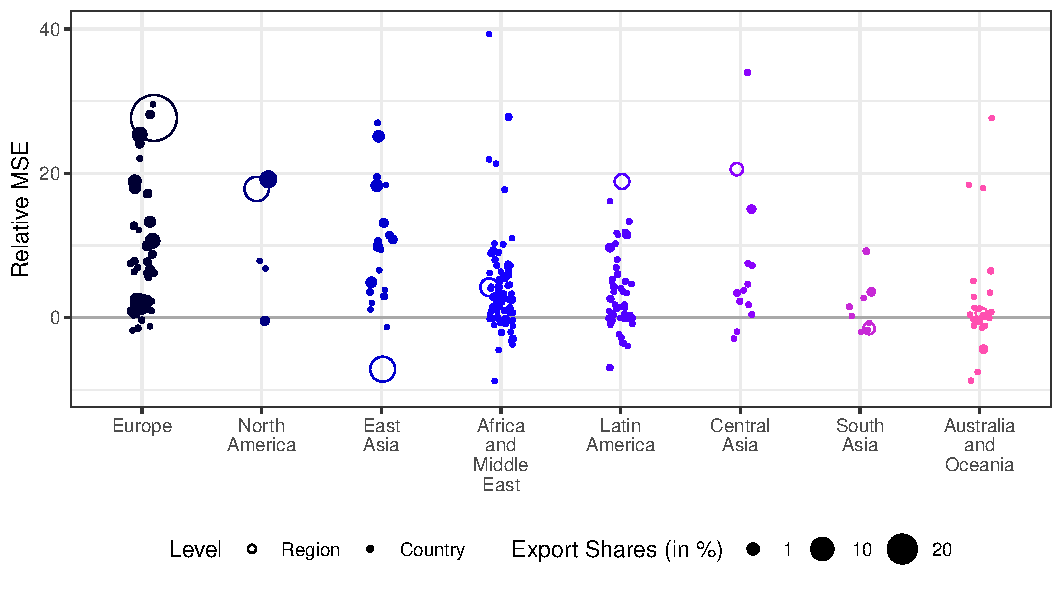
\includegraphics[width=\textwidth]{fig/fig_eval_regions}
	\caption[Relative Accuracy of Reconciliation Methods by Regions]{\textbf{Relative Accuracy of Reconciliation Methods by Regions.} \small{\textit{Higher points indicate better forecasts. Zero line shows the accuracy of unreconciled predictions. Reconciliation using unweighted BSR.}}}\label{fig:eval_regions}
\end{figure}
The same results also hold true for the relative forecast accuracy by categories, as shown in figure \ref{fig:eval_categories}. Because the export shares in the categorical hierarchy are more evenly distributed, the pattern of smaller export volumes being worse off due to reconciliation is less pronounced. The results for other variance scaling methods such as weighted least squares and MinT are very similar.
\begin{figure}[H]
	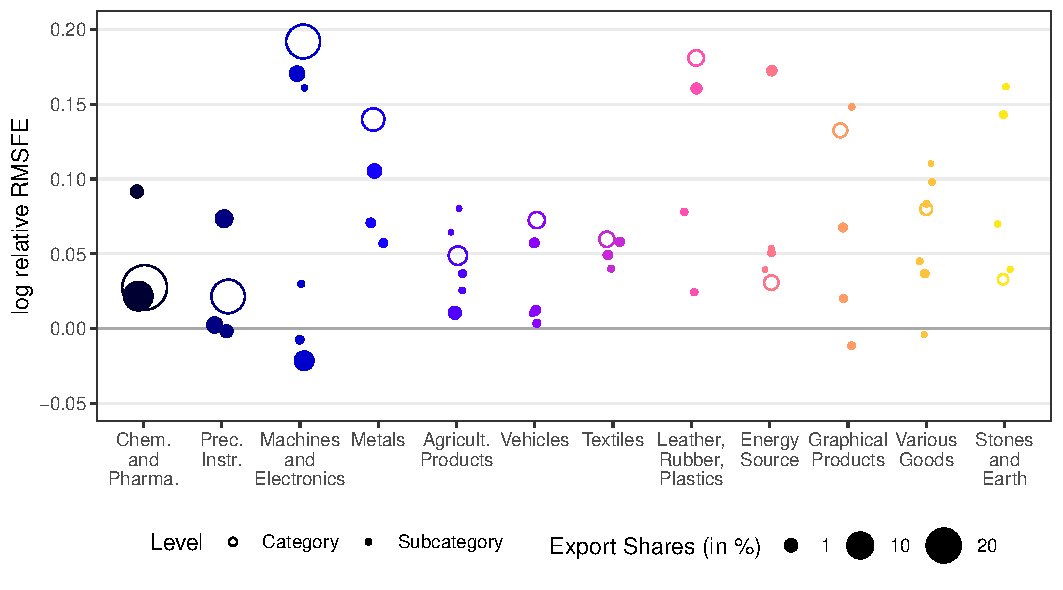
\includegraphics[width=\textwidth]{fig/fig_eval_categories}
	\caption[Relative Accuracy of Reconciliation Methods by Categories]{\textbf{Relative Accuracy of Reconciliation Methods by Categories.} \small{\textit{Higher points indicate better forecasts. Zero line shows the accuracy of unreconciled predictions. Reconciliation using unweighted BSR.}}}\label{fig:eval_categories}
\end{figure}




\subsection{Benefits of Weighting}\label{sec:resweight}
An advantage of the general weighting scheme is that selected series can be shrunk towards their base forecast. This is particularly useful if there exists judgmental information for a specific forecast that would require adjustments for all other base forecasts in a hierarchy. An example is the reclassification of electricity as a good instead of a service. Figure \ref{fig:fcex} shows total exports of energy sources for unweighted and weighted reconciliation.
\begin{figure}[H]
	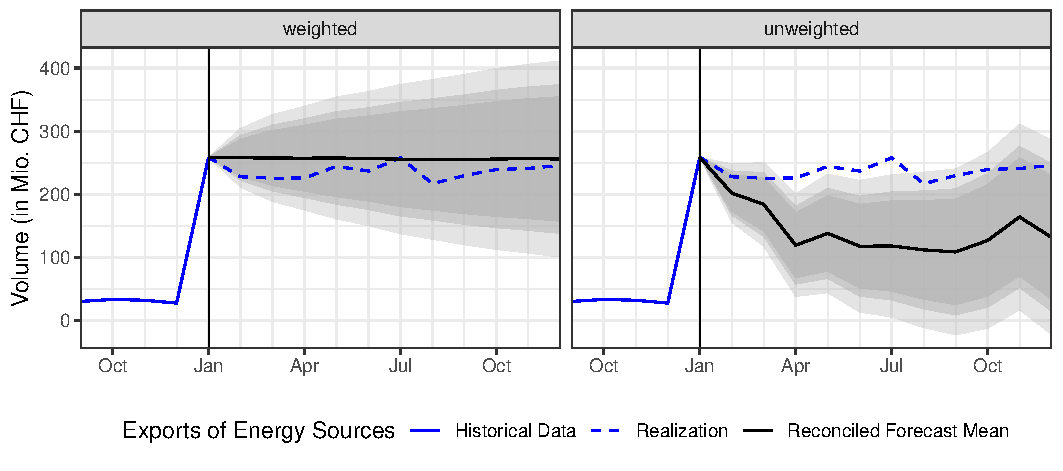
\includegraphics[width=\textwidth]{fig/fig_electricity}
	\caption[Forecast with Bias Weighting]{\small{\textbf{Forecast with Bias Weighting}. \textit{Left panel shows weighted, right panel unweighted reconciliation with identical random walk base forecast for energy exports. Grey ribbons indicate 90\%, 95\% and 99\% prediction intervals.}}}\label{fig:fcex}
\end{figure}
After observing the first value including electric energy in January 2002, a random walk forecast is used for this particular series. Then the series are reconciled with and without an appropriate weighting scheme. For the unweighted model on the right, the other base forecasts assume the structural break to be an outlier and dominate the information from the random walk forecast. Even though the forecaster has prior knowledge that the random walk forecast is accurate, it is overruled in the reconciliation procedure. The only way out would be to adjust the base forecasts for all other series as well, which is very cumbersome.

The model on the left shows the reconciliation of the same forecasts with more weight on the random walk forecast. This is done as described in subsection \ref{sec:weighting}. The diagonal entry in $\Lambda$ that corresponds to the random walk forecast is scaled down. At the same time, the remaining entries are scaled up such that the determinant of $\Lambda$ remains at 1. This forces the reconciled forecast for energy sources to stay close to its random walk base forecast. The remaining series adjust accordingly during the reconciliation procedure. As a result, the mean squared error of the forecast for energy sources in 2002 is more than 90\% lower than in the unweighted case. This also leads to substantial accuracy gains at other levels, while only a few forecast are less accurate. The forecast for total exports for instance is 14\% more accurate.

The prediction intervals are drawn from the conditional posterior distribution of $\Sigma$ and depend therefore on the predictive distributions of the base forecasts. Since the intervals generated by the underlying models tend to be too narrow, the prediction intervals for the reconciled forecasts are too optimistic as well. This issue could be addressed using models more suited for density forecasts or bootstrap aggregation of the exponential smoothing methods \citep{Bergmeir2016}.\\

\section{Conclusion}\label{sec:conc}
This paper extends the existing literature on hierarchical forecast combination by establishing a Bayesian estimation framework and introducing an explicit definition of the reconciliation bias. This leads to several innovations: It is possible to use prior subjective judgment of the forecaster to shrink reconciled forecasts towards their corresponding base forecasts. The Bayesian sampling procedure allows the incorporation of prior information on the parameters in order to avoid some issues such as the occurrence of negative reconciled forecasts. The use of predictive densities allows for greater flexibility in the choice of the base forecast models, taking for instance conditional heteroskedasticity into account when weighting the forecasts at different horizons. However, because the approach requires repeated sampling from the joint posterior distribution, it tends to be slower than established reconciliation techniques.

Using a comprehensive dataset of Swiss goods exports, this paper demonstrates that optimal combination methods using variance scaling improve the forecasting accuracy significantly compared to the unreconciled case and simpler reconciliation methods. The results are robust to changes in the forecasting horizon, the underlying base forecast models and the measure used to determine forecasting accuracy. Optimal combination methods are shown to be particularly useful in the case of misspecified models, during periods of high volatility in the time series and for projections that extend further into the future. Even though the forecasting accuracy is significantly better on average, no reconciliation method consistently outperforms the unreconciled forecasts across the hierarchy or over time. Forecasts at the top of level tend to benefit more from reconciliation than the noisy series at the bottom of a hierarchy. At the same level in a hierarchy, forecasts that account for a larger share of the total are on average more accurate after reconciliation. The paper has also provided an example where weighting based on subjective judgment can significantly improve forecasting performance. 



\clearpage

% bibliography
\pagenumbering{Roman}
\setcounter{page}{2}
\bibliography{library}
\bibliographystyle{apalike}

\clearpage


% appendix

\appendix
\section{Appendix}


\subsection{Robustness}
\label{sec:robust}

\begin{figure}[H]
	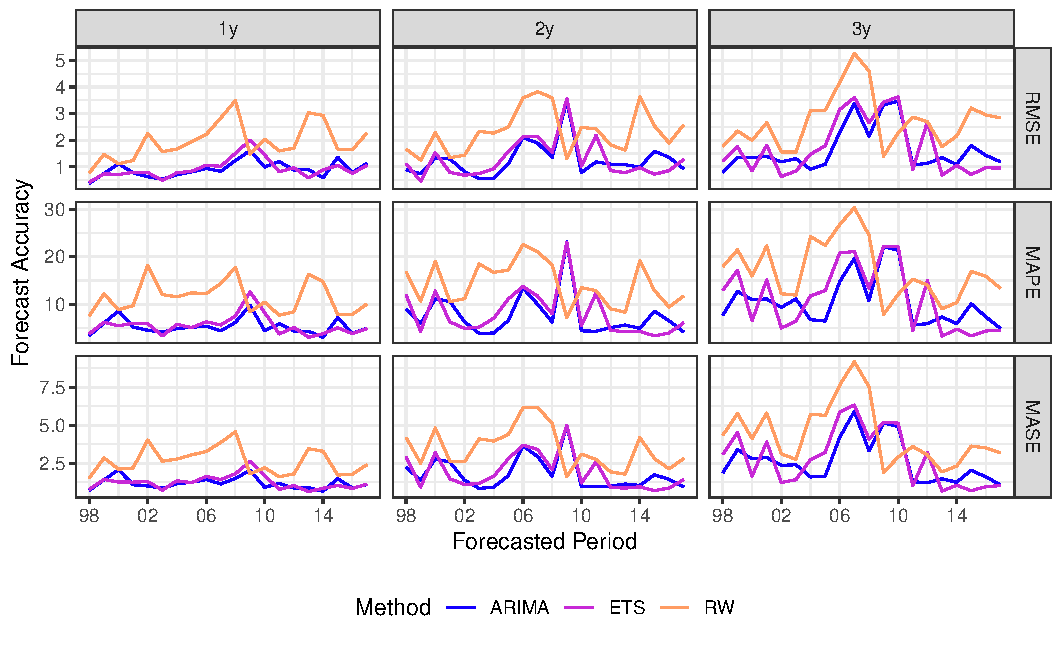
\includegraphics[width=\textwidth]{fig/fig_eval_methods_top}
	\caption{Accuracy of Forecasting Methods at the Top Level}
\end{figure}

\begin{figure}[H]
	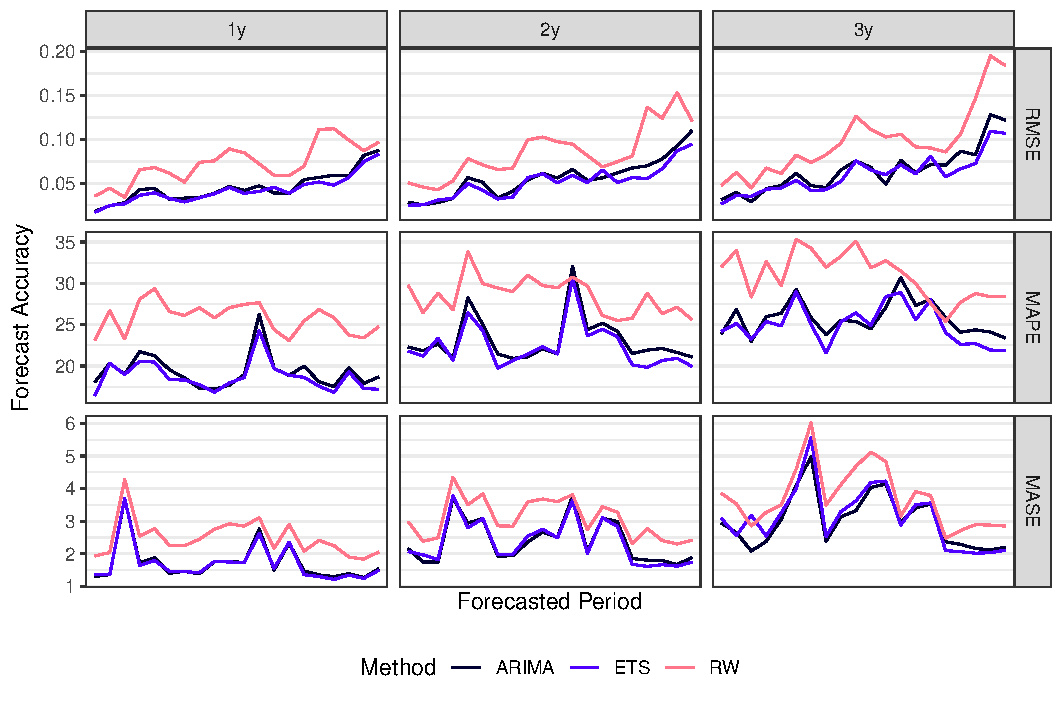
\includegraphics[width=\textwidth]{fig/fig_eval_methods_bottom}
	\caption{Accuracy of Forecasting Methods at the Bottom Level}
\end{figure}


\subsection{Data}
\label{sec:data}
The data is compiled by the Swiss Federal Customs Administration\footnote{\url{https://www.ezv.admin.ch/ezv/en/home/topics/swiss-foreign-trade-statistics.html}} and made available in a machine-friendly format on basis of a subscription.\\
% table with goods categories
\begin{small}
\begin{longtable}{p{2.5cm}p{11.5cm}}
\caption{Tariff Numbers and Descriptions of Goods}\\
\toprule
\normalsize{Tariff Number} & \normalsize{Description}\\
\midrule
\endfirsthead
\multicolumn{2}{@{}l}{\ldots continued}\\
\toprule
\normalsize{Tariff Number} & \normalsize{Description}\\  
\midrule
\endhead
\bottomrule
\multicolumn{2}{r@{}}{continued \ldots}\\
\endfoot
\bottomrule
\endlastfoot
	01	&	Forestry and agricultural products, fisheries	\\
\enskip	01.1	&	Food, beverages and tobacco	\\
\enskip	01.2	&	Feeding stuffs for animals	\\
\enskip	01.3	&	Live animals	\\
\enskip	01.4	&	Horticultural products	\\
\enskip	01.5	&	Forestry products (not firewood)	\\
\enskip	01.6	&	Products for commercial/industrial further processing such as oils, fats, starches, plants and vegetable parts, etc.	\\
\midrule
	02	&	Energy source	\\
\enskip	02.1	&	Solid combustibles	\\
\enskip	02.2	&	Petroleum and distillates	\\
\enskip	02.3	&	Gas	\\
\enskip	02.4	&	Electrical energy	\\
\midrule
	03	&	Textiles, clothing, shoes	\\
\enskip	03.1	&	Textiles	\\
\enskip	03.2	&	Articles of apparel and clothing	\\
\enskip	03.3	&	Shoes, parts and accessories	\\
\midrule
	04	&	Paper, articles of paper and and products of the printing industry	\\
\enskip	04.1	&	Basic materials for paper production, such as cellulose and cellulose fibre and paper and carton waste	\\
\enskip	04.2	&	Paper and carton in rolls, strips or sheets	\\
\enskip	04.3	&	Goods from paper or carton	\\
\enskip	04.4	&	Products of the printing industry	\\
\midrule
	05	&	Leather, rubber, plastics	\\
\enskip	05.1	&	Leather	\\
\enskip	05.2	&	Rubber	\\
\enskip	05.3	&	Plastics	\\
\midrule
	06	&	Products of the chemical and pharmaceutical industry	\\
\enskip	06.1	&	Chemical raw materials, basic materials and unformed plastics	\\
\enskip	06.2	&	Chemical end products, vitamins, diagnostic products, including active substances	\\
\midrule
	07	&	Stones and earth	\\
\enskip	07.1	&	Mineral raw materials and basic products	\\
\enskip	07.2	&	Goods from stone and cement	\\
\enskip	07.3	&	Ceramic wares	\\
\enskip	07.4	&	Glass	\\
\midrule
	08	&	Metals	\\
\enskip	08.1	&	Iron and steel	\\
\enskip	08.2	&	Non-ferrous metals	\\
\enskip	08.3	&	Metal goods	\\
\midrule
	09	&	Machines, appliances, electronics	\\
\enskip	09.1	&	Industrial machinery	\\
\enskip	09.2	&	Agricultural machines	\\
\enskip	09.3	&	Household appliances	\\
\enskip	09.4	&	Office machines	\\
\enskip	09.5	&	Electrical and electronic industry appliances and devices	\\
\enskip	09.6	&	Military equipment	\\
\midrule
	10	&	Vehicles	\\
\enskip	10.1	&	Road vehicles	\\
\enskip	10.2	&	Railed vehicles	\\
\enskip	10.3	&	Air- and spacecraft	\\
\enskip	10.4	&	Watercraft	\\
\midrule
	11	&	Precision instruments, clocks and watches and jewellery	\\
\enskip	11.1	&	Precision instruments and equipment	\\
\enskip	11.2	&	Watches	\\
\enskip	11.3	&	Jewellery and household goods made from precious metals	\\
\midrule
	12	&	Various goods such as music instruments, home furnishings, toys, sports equipment, etc.	\\
\enskip	12.1	&	Exposed film	\\
\enskip	12.2	&	Music instruments	\\
\enskip	12.3	&	Home furnishings	\\
\enskip	12.4	&	Toys and sports equipment	\\
\enskip	12.5	&	Stationery goods	\\
\enskip	12.6	&	Various goods such as umbrellas, neon signs, festive articles, brushes, lighters, pipes, etc.	\\
\midrule
	13	&	Precious metals, precious and semi-precious stones	\\
\enskip	13.1	&	Precious and semi-precious stones	\\
\enskip	13.2	&	Precious metals (including gold and silver bars from 1.1.2012)	\\
\midrule
	14	&	Works of art and antiques	\\
\enskip	14.1	&	Works of art	\\
\enskip	14.2	&	Antiques and collectors' items	\\
\end{longtable}
\end{small}

\clearpage

\begin{small}
	\begin{longtable}{p{7.5cm}cccc}
		\caption{Countries and Regional Aggregates}\\
		\toprule
Country	&	isoCode	&	regCode	&	valid from	&	valid to	\\
		\midrule
		\endfirsthead
		\multicolumn{4}{@{}l}{\ldots continued}\\
		\toprule
Country	&	isoCode	&	regCode	&	valid from	&	valid to	\\
		\midrule
		\endhead
		\bottomrule
		\multicolumn{4}{r@{}}{continued \ldots}\\
		\endfoot
		\bottomrule
		\endlastfoot
Switzerland	&	CH	&	EU	&	01/1988	&	-	\\
Germany	&	DE	&	EU	&	01/1988	&	-	\\
France	&	FR	&	EU	&	01/1988	&	-	\\
Italy	&	IT	&	EU	&	01/1988	&	-	\\
Netherlands	&	NL	&	EU	&	01/1988	&	-	\\
Belgium-Luxembourg	&	BE	&	EU	&	01/1988	&	12/1998	\\
Belgium	&	BE	&	EU	&	01/1999	&	-	\\
Luxembourg	&	LU	&	EU	&	01/1999	&	-	\\
Austria	&	AT	&	EU	&	01/1988	&	-	\\
United Kingdom	&	GB	&	EU	&	01/1988	&	-	\\
Denmark	&	DK	&	EU	&	01/1988	&	-	\\
Norway	&	NO	&	EU	&	01/1988	&	-	\\
Sweden	&	SE	&	EU	&	01/1988	&	-	\\
Portugal	&	PT	&	EU	&	01/1988	&	-	\\
Finland	&	FI	&	EU	&	01/1988	&	-	\\
Croatia, Republic of	&	HR	&	EU	&	02/1992	&	-	\\
Slovenia	&	SI	&	EU	&	02/1992	&	-	\\
Bosnia and Herzegovina	&	BA	&	EU	&	05/1992	&	-	\\
Macedonia	&	MK	&	EU	&	05/1992	&	-	\\
Montenegro	&	ME	&	EU	&	05/1992	&	12/1996	\\
Montenegro	&	ME	&	EU	&	01/2007	&	-	\\
Montenegro	&	XM	&	EU	&	01/2006	&	12/2006	\\
Serbia	&	SQ	&	EU	&	05/1992	&	12/1996	\\
Serbia	&	RS	&	EU	&	01/2007	&	-	\\
Serbia	&	XS	&	EU	&	01/2006	&	12/2006	\\
Federal Republic of Yugoslavia	&	YU	&	EU	&	01/1997	&	12/2003	\\
Serbia and Montenegro	&	CS	&	EU	&	01/2004	&	12/2005	\\
Kosovo	&	XK	&	EU	&	01/2006	&	-	\\
Iceland	&	IS	&	EU	&	01/1988	&	-	\\
Ireland	&	IE	&	EU	&	01/1988	&	-	\\
Spain	&	ES	&	EU	&	01/1988	&	-	\\
Greece	&	GR	&	EU	&	01/1988	&	-	\\
Turkey	&	TR	&	EU	&	01/1988	&	-	\\
GDR	&	DD	&	EU	&	01/1988	&	10/1990	\\
Poland	&	PL	&	EU	&	01/1988	&	-	\\
Czech Republic	&	CZ	&	EU	&	01/1993	&	-	\\
Czechoslovakia	&	CS	&	EU	&	01/1988	&	02/1992	\\
Slovakia	&	SK	&	EU	&	01/1993	&	-	\\
Hungary	&	HU	&	EU	&	01/1988	&	-	\\
Albania	&	AL	&	EU	&	01/1988	&	-	\\
Bulgaria, Republic of	&	BG	&	EU	&	01/1988	&	-	\\
Romania	&	RO	&	EU	&	01/1988	&	-	\\
USSR	&	SU	&	EU	&	01/1988	&	12/1991	\\
Yugoslavia	&	YU	&	EU	&	01/1988	&	04/1992	\\
Cyprus	&	CY	&	EU	&	01/1988	&	-	\\
Svalbard and Jan Mayen Island	&	SJ	&	EU	&	01/1999	&	-	\\
Malta	&	MT	&	EU	&	01/1988	&	-	\\
Gibraltar	&	GI	&	EU	&	01/1988	&	-	\\
Faeroe Islands	&	FO	&	EU	&	01/1988	&	-	\\
San Marino	&	SM	&	EU	&	01/1999	&	-	\\
Holy See	&	VA	&	EU	&	01/1999	&	-	\\
Andorra	&	AD	&	EU	&	01/1988	&	-	\\
Estonia	&	EE	&	EU	&	01/1992	&	-	\\
Latvia	&	LV	&	EU	&	01/1992	&	-	\\
Lithuania	&	LT	&	EU	&	01/1992	&	-	\\
Russian Federation	&	RU	&	CA	&	01/1992	&	-	\\
Armenia	&	AM	&	CA	&	01/1992	&	-	\\
Azerbaijan	&	AZ	&	CA	&	01/1992	&	-	\\
Belarus	&	BY	&	CA	&	01/1992	&	-	\\
Georgia	&	GE	&	CA	&	01/1992	&	-	\\
Kazakhstan	&	KZ	&	CA	&	01/1992	&	-	\\
Kyrgyz, Republic	&	KG	&	CA	&	01/1992	&	-	\\
Moldova, Republic of	&	MD	&	CA	&	01/1992	&	-	\\
Tajikistan	&	TJ	&	CA	&	01/1992	&	-	\\
Turkmenistan	&	TM	&	CA	&	01/1992	&	-	\\
Ukraine	&	UA	&	CA	&	01/1992	&	-	\\
Uzbekistan	&	UZ	&	CA	&	01/1992	&	-	\\
Egypt	&	EG	&	AF	&	01/1988	&	-	\\
Sudan	&	SD	&	AF	&	01/1988	&	-	\\
South Sudan, Republic of	&	SS	&	AF	&	09/2011	&	-	\\
Libya	&	LY	&	AF	&	01/1988	&	-	\\
Tunisia	&	TN	&	AF	&	01/1988	&	-	\\
Algeria	&	DZ	&	AF	&	01/1988	&	-	\\
Canary Islands	&	XA	&	AF	&	01/1988	&	-	\\
Morocco	&	MA	&	AF	&	01/1988	&	-	\\
Western Sahara	&	EH	&	AF	&	01/1999	&	-	\\
Ceuta and Melilla	&	XB	&	AF	&	01/1988	&	12/2010	\\
Equatorial Guinea	&	GQ	&	AF	&	01/1988	&	-	\\
Ceuta	&	XC	&	AF	&	01/2001	&	-	\\
Melilla	&	XL	&	AF	&	01/2001	&	-	\\
Togo	&	TG	&	AF	&	01/1988	&	-	\\
Senegal	&	SN	&	AF	&	01/1988	&	-	\\
Mali	&	ML	&	AF	&	01/1988	&	-	\\
Mauritania	&	MR	&	AF	&	01/1988	&	-	\\
Côte d'Ivoire	&	CI	&	AF	&	01/1988	&	-	\\
Burkina Faso	&	BF	&	AF	&	01/1988	&	-	\\
Benin	&	BJ	&	AF	&	01/1988	&	-	\\
Niger	&	NE	&	AF	&	01/1988	&	-	\\
Guinea	&	GN	&	AF	&	01/1988	&	-	\\
Gambia	&	GM	&	AF	&	01/1988	&	-	\\
Sierra Leone	&	SL	&	AF	&	01/1988	&	-	\\
Liberia	&	LR	&	AF	&	01/1988	&	-	\\
Ghana	&	GH	&	AF	&	01/1988	&	-	\\
Nigeria, Federal Republic of	&	NG	&	AF	&	01/1988	&	-	\\
Cameroon	&	CM	&	AF	&	01/1988	&	-	\\
Gabon	&	GA	&	AF	&	01/1988	&	-	\\
Congo, Republic of the	&	CG	&	AF	&	01/1988	&	-	\\
Central African Republic	&	CF	&	AF	&	01/1988	&	-	\\
Chad	&	TD	&	AF	&	01/1988	&	-	\\
Congo, Democratic Republic of the	&	CD	&	AF	&	06/1997	&	-	\\
Zaire	&	ZR	&	AF	&	01/1988	&	05/1997	\\
Angola	&	AO	&	AF	&	01/1988	&	-	\\
Guinea-Bissau	&	GW	&	AF	&	01/1988	&	-	\\
Botswana	&	BW	&	AF	&	01/1988	&	-	\\
Cabo Verde, Republic of	&	CV	&	AF	&	01/1988	&	-	\\
Lesotho	&	LS	&	AF	&	01/1988	&	-	\\
Sao Tomé and Principe	&	ST	&	AF	&	01/1988	&	-	\\
Namibia	&	NA	&	AF	&	01/1988	&	-	\\
South Africa	&	ZA	&	AF	&	01/1988	&	-	\\
Swaziland	&	SZ	&	AF	&	01/1988	&	-	\\
Zambia	&	ZM	&	AF	&	01/1988	&	-	\\
Zimbabwe	&	ZW	&	AF	&	01/1988	&	-	\\
Malawi	&	MW	&	AF	&	01/1988	&	-	\\
Mozambique	&	MZ	&	AF	&	01/1988	&	-	\\
Madagascar, Republic of	&	MG	&	AF	&	01/1988	&	-	\\
Réunion	&	RE	&	AF	&	01/1988	&	-	\\
St Helena, Ascen. and Tristan da Cunha	&	SH	&	AF	&	01/1988	&	-	\\
Comoros, Union of	&	KM	&	AF	&	01/1988	&	-	\\
Antarctica	&	AQ	&	AF	&	01/1988	&	-	\\
Mauritius	&	MU	&	AF	&	01/1988	&	-	\\
British Indian Ocean Territory	&	IO	&	AF	&	01/1988	&	-	\\
Tanzania, United Republic of	&	TZ	&	AF	&	01/1988	&	-	\\
Seychelles, Republic of	&	SC	&	AF	&	01/1988	&	-	\\
Rwanda	&	RW	&	AF	&	01/1988	&	-	\\
Bouvet Island	&	BV	&	AF	&	01/1999	&	-	\\
Burundi	&	BI	&	AF	&	01/1988	&	-	\\
Mayotte	&	YT	&	AF	&	01/1999	&	-	\\
Somalia, Federal Republic of	&	SO	&	AF	&	01/1988	&	-	\\
French Southern Territories	&	TF	&	AF	&	01/1999	&	-	\\
Djibouti	&	DJ	&	AF	&	01/1988	&	-	\\
Eritrea	&	ER	&	AF	&	01/1994	&	-	\\
Ethiopia, Fed. Democratic Republic of	&	ET	&	AF	&	01/1988	&	-	\\
Kenya	&	KE	&	AF	&	01/1988	&	-	\\
Uganda	&	UG	&	AF	&	01/1988	&	-	\\
Syrian Arab Republic	&	SY	&	AF	&	01/1988	&	-	\\
Lebanon	&	LB	&	AF	&	01/1988	&	-	\\
Israel	&	IL	&	AF	&	01/1988	&	-	\\
Palestine, the State of	&	PS	&	AF	&	01/1997	&	-	\\
Jordan	&	JO	&	AF	&	01/1988	&	-	\\
Saudi Arabia	&	SA	&	AF	&	01/1988	&	-	\\
Yemen (Nord)	&	YE	&	AF	&	01/1988	&	12/1990	\\
Yemen	&	YE	&	AF	&	01/1991	&	-	\\
Yemen (Sud)	&	YD	&	AF	&	01/1988	&	12/1990	\\
Qatar	&	QA	&	AF	&	01/1988	&	-	\\
Bahrain	&	BH	&	AF	&	01/1988	&	-	\\
United Arab Emirates	&	AE	&	AF	&	01/1988	&	-	\\
Oman	&	OM	&	AF	&	01/1988	&	-	\\
Kuwait	&	KW	&	AF	&	01/1988	&	-	\\
Iraq	&	IQ	&	AF	&	01/1988	&	-	\\
Iran, Islamic Republic of	&	IR	&	AF	&	01/1988	&	-	\\
Afghanistan	&	AF	&	SA	&	01/1988	&	-	\\
Pakistan	&	PK	&	SA	&	01/1988	&	-	\\
Bangladesh	&	BD	&	SA	&	01/1988	&	-	\\
India	&	IN	&	SA	&	01/1988	&	-	\\
Sri Lanka	&	LK	&	SA	&	01/1988	&	-	\\
Maldives	&	MV	&	SA	&	01/1988	&	-	\\
Nepal, Federal Democratic Rep.	&	NP	&	SA	&	01/1988	&	-	\\
Bhutan	&	BT	&	SA	&	01/1988	&	-	\\
Myanmar, Union of	&	MM	&	EA	&	01/1988	&	-	\\
Thailand	&	TH	&	EA	&	01/1988	&	-	\\
Malaysia	&	MY	&	EA	&	01/1988	&	-	\\
Brunei Darussalam	&	BN	&	EA	&	01/1988	&	-	\\
Singapore	&	SG	&	EA	&	01/1988	&	-	\\
Cambodia	&	KH	&	EA	&	01/1988	&	-	\\
Lao, People's Democratic Republic	&	LA	&	EA	&	01/1988	&	-	\\
Viet Nam, Socialist Republic of	&	VN	&	EA	&	01/1988	&	-	\\
Mongolia	&	MN	&	EA	&	01/1988	&	-	\\
China, People's Republic of	&	CN	&	EA	&	01/1988	&	-	\\
Hong Kong	&	HK	&	EA	&	01/1988	&	-	\\
Taiwan	&	TW	&	EA	&	01/1988	&	-	\\
Macau	&	MO	&	EA	&	01/1988	&	-	\\
Korea, People's Democratic Republic of	&	KP	&	EA	&	01/1988	&	-	\\
Korea, Republic of	&	KR	&	EA	&	01/1988	&	-	\\
Japan	&	JP	&	EA	&	01/1988	&	-	\\
Philippines	&	PH	&	EA	&	01/1988	&	-	\\
Indonesia	&	ID	&	EA	&	01/1988	&	-	\\
East Timor	&	TL	&	EA	&	01/2004	&	-	\\
East Timor	&	TP	&	EA	&	01/1999	&	12/2003	\\
Canada	&	CA	&	NA	&	01/1988	&	-	\\
St Pierre and Miquelon	&	PM	&	NA	&	01/1988	&	-	\\
United States	&	US	&	NA	&	01/1988	&	-	\\
Greenland	&	GL	&	NA	&	01/1988	&	-	\\
Mexico	&	MX	&	LA	&	01/1988	&	-	\\
Belize	&	BZ	&	LA	&	01/1988	&	-	\\
Guatemala	&	GT	&	LA	&	01/1988	&	-	\\
Honduras	&	HN	&	LA	&	01/1988	&	-	\\
El Salvador	&	SV	&	LA	&	01/1988	&	-	\\
Nicaragua	&	NI	&	LA	&	01/1988	&	-	\\
Costa Rica	&	CR	&	LA	&	01/1988	&	-	\\
Panama	&	PA	&	LA	&	01/1988	&	-	\\
Cayman Islands	&	KY	&	LA	&	01/1988	&	-	\\
Turks and Caicos Islands	&	TC	&	LA	&	01/1988	&	-	\\
Bahamas	&	BS	&	LA	&	01/1988	&	-	\\
Bermuda	&	BM	&	LA	&	01/1988	&	-	\\
Jamaica	&	JM	&	LA	&	01/1988	&	-	\\
Cuba	&	CU	&	LA	&	01/1988	&	-	\\
Haiti	&	HT	&	LA	&	01/1988	&	-	\\
Dominican Republic	&	DO	&	LA	&	01/1988	&	-	\\
American Virgin Islands	&	VI	&	LA	&	01/1988	&	-	\\
Puerto Rico	&	PR	&	LA	&	01/1988	&	12/2005	\\
Dominica	&	DM	&	LA	&	01/1988	&	-	\\
St Vincent and the Grenadines	&	VC	&	LA	&	01/1988	&	-	\\
St Lucia	&	LC	&	LA	&	01/1988	&	-	\\
Montserrat	&	MS	&	LA	&	01/1988	&	-	\\
Antigua and Barbuda	&	AG	&	LA	&	01/1988	&	-	\\
Barbados	&	BB	&	LA	&	01/1988	&	-	\\
Grenada	&	GD	&	LA	&	01/1988	&	-	\\
St Kitts and Nevis	&	KN	&	LA	&	01/1988	&	-	\\
Anguilla	&	AI	&	LA	&	01/1988	&	-	\\
Guadeloupe	&	GP	&	LA	&	01/1988	&	-	\\
British Virgin Islands	&	VG	&	LA	&	01/1999	&	-	\\
Martinique	&	MQ	&	LA	&	01/1988	&	-	\\
Trinidad and Tobago	&	TT	&	LA	&	01/1988	&	-	\\
Saint BarthÈlemy	&	BL	&	LA	&	01/2013	&	-	\\
Netherlands Antilles	&	AN	&	LA	&	01/1988	&	12/2012	\\
Aruba	&	AW	&	LA	&	01/1999	&	-	\\
Bonaire, Sint Eustatius and Saba	&	BQ	&	LA	&	01/2013	&	-	\\
Curacao	&	CW	&	LA	&	01/2013	&	-	\\
Sint Maarten (NL)	&	SX	&	LA	&	01/2013	&	-	\\
Colombia	&	CO	&	LA	&	01/1988	&	-	\\
Venezuela, the Bolivarian Republic of	&	VE	&	LA	&	01/1988	&	-	\\
Guyana	&	GY	&	LA	&	01/1988	&	-	\\
Suriname	&	SR	&	LA	&	01/1988	&	-	\\
French Guiana	&	GF	&	LA	&	01/1988	&	-	\\
Brazil	&	BR	&	LA	&	01/1988	&	-	\\
Paraguay	&	PY	&	LA	&	01/1988	&	-	\\
Uruguay	&	UY	&	LA	&	01/1988	&	-	\\
Argentina	&	AR	&	LA	&	01/1988	&	-	\\
Falkland Islands	&	FK	&	LA	&	01/1988	&	-	\\
South Georgia and South Sandwich Islands	&	GS	&	LA	&	01/1999	&	-	\\
Chile	&	CL	&	LA	&	01/1988	&	-	\\
Bolivia, the Plurinational State of	&	BO	&	LA	&	01/1988	&	-	\\
Peru	&	PE	&	LA	&	01/1988	&	-	\\
Ecuador	&	EC	&	LA	&	01/1988	&	-	\\
Australia	&	AU	&	AO	&	01/1988	&	-	\\
Papua New Guinea	&	PG	&	AO	&	01/1988	&	-	\\
Cocos (Keeling) Islands	&	CC	&	AO	&	01/1999	&	-	\\
Heard and McDonald Islands	&	HM	&	AO	&	01/1999	&	-	\\
Norfolk Island	&	NF	&	AO	&	01/1999	&	-	\\
Christmas Island	&	CX	&	AO	&	01/1999	&	-	\\
New Zealand	&	NZ	&	AO	&	01/1988	&	-	\\
Cook Islands	&	CK	&	AO	&	01/1998	&	-	\\
Samoa	&	WS	&	AO	&	01/1988	&	-	\\
Niue Island	&	NU	&	AO	&	01/1999	&	-	\\
Kiribati, the Republic of	&	KI	&	AO	&	01/1988	&	-	\\
Tokelau Islands	&	TK	&	AO	&	01/1999	&	-	\\
Tuvalu	&	TV	&	AO	&	01/1988	&	-	\\
Pitcairn Islands	&	PN	&	AO	&	01/1988	&	-	\\
Solomon Islands	&	SB	&	AO	&	01/1988	&	-	\\
French Polynesia	&	PF	&	AO	&	01/1988	&	-	\\
New Caledonia	&	NC	&	AO	&	01/1999	&	-	\\
Wallis and Futuna	&	WF	&	AO	&	01/1999	&	-	\\
American Oceania	&	PU	&	AO	&	01/1988	&	12/1996	\\
American Oceania	&	UM	&	AO	&	01/2006	&	-	\\
American Oceania	&	UM	&	AO	&	01/1997	&	12/2005	\\
Northern Mariana, Islands	&	MP	&	AO	&	01/1997	&	-	\\
Marshall Islands	&	MH	&	AO	&	01/1997	&	-	\\
Micronesia, Federated States of	&	FM	&	AO	&	01/1997	&	-	\\
Palau	&	PW	&	AO	&	01/1997	&	-	\\
Fiji, Republic of	&	FJ	&	AO	&	01/1988	&	-	\\
American Samoa	&	AS	&	AO	&	01/2006	&	-	\\
Guam	&	GU	&	AO	&	01/2006	&	-	\\
Vanuatu	&	VU	&	AO	&	01/1988	&	-	\\
Nauru	&	NR	&	AO	&	01/1988	&	-	\\
Tonga	&	TO	&	AO	&	01/1988	&	-	\\
Countries not specified	&	QX	&	EU	&	01/2002	&	-	\\
\end{longtable}
\end{small}

\subsection{Scaling Methods}
\label{subsec:scaling}
by equation (\ref{eq:scale}).
\begin{align}
	\label{eq:scale}
	|\lambda| &= \lambda_1 \lambda_2 \hdots \lambda_m
	= \prod_{s^- = 1}^{x} \lambda_{s^-}\ \eta^{-\frac{1}{x}}   \prod_{s^+ = x+1}^{m} \lambda_{s^+}\ \eta^{\frac{1}{m-x}} = 1
\end{align}
The $x$ local variance components $\lambda_{s^-}$ are scaled down by a factor $\eta^{\frac{1}{x}}$ and the remaining $(m-x)$ components $\lambda_{s^+}$ are correspondingly scaled up by a factor $\eta^{\frac{1}{m-x}}$. The generalized variance remains at unity irrespective of the scaling factor $\eta$ and the number of series to be scaled down $x$. 





\end{document}